%% =====================================================================
%% Documento de Planejamento do Projeto — Entrega 01 (29/08/2026)
%% Experiência Criativa: Projeto Transformador II — BCC / PUCPR
%% Autora: Gabriela Sofia
%% Formatação: IEEEtran conference (padrão do template dos professores)
%% Compilar: pdflatex main && pdflatex main
%% Versão: v10 (2026-08-20) — E4 passa a concluída (holdout temporal sobre a
%% tabela única, MOD-PROSP-02); v9 (2026-08-18) — delta real do planejamento02.pdf contra o v8
%% real (não a v4 que ele já tinha gerado): gloss em PT-BR de "payload",
%% reprodutibilidade amarrada ao ambiente do projeto, propósito explícito no
%% cronograma, parágrafo de integração reordenado. Ver NOTA_versoes.md §12
%% para o detalhe nota a nota.
%% =====================================================================
\documentclass[conference]{IEEEtran}
\IEEEoverridecommandlockouts

\usepackage[T1]{fontenc}
\usepackage[utf8]{inputenc}
\usepackage[brazil]{babel}
\usepackage{graphicx}
\usepackage{booktabs}
\usepackage{array}
\usepackage{amsmath,amssymb}
\usepackage{xcolor}
\usepackage{tikz}
\usetikzlibrary{arrows.meta,positioning,fit,backgrounds,shapes.misc}
\usepackage{cite}
\usepackage{url}
\usepackage[hidelinks]{hyperref}

% cores do diagrama
\definecolor{cAzul}{HTML}{1F4E79}
\definecolor{cVerm}{HTML}{C0504D}
\definecolor{cVerd}{HTML}{3F6F4A}
\definecolor{cCinz}{HTML}{7F7F7F}
\definecolor{cFundo}{HTML}{EEF3F8}
\definecolor{cFundoAux}{HTML}{F7F0EE}
\definecolor{cFundoPrd}{HTML}{EDF3EE}

\begin{document}

\title{Suscetibilidade urbana a enchentes com base causal
físico-hidrológica: da evidência heterogênea ao serviço de inferência
auditável}

\author{\IEEEauthorblockN{Gabriela Sofia}
\IEEEauthorblockA{Experiência Criativa: Projeto Transformador II\\
Bacharelado em Ciência da Computação --- PUCPR\\
Turma \textcolor{red}{7A} --- Equipe \textcolor{red}{N}\\
\{\texttt{gabriela.milani}\}@pucpr.edu.br}}

\maketitle

% =====================================================================
\section{Descrição do Projeto}

Enchentes, alagamentos e deslizamentos são o desastre de maior recorrência no
Brasil, e atingem primeiro quem não escolheu onde morar. Relevo que não escoa
a água e relevo que cede sob ela são duas faces da mesma vulnerabilidade
física; da hostilidade desse relevo nasce a ocupação urbana precária, e dela,
a vulnerabilidade social. Entre 2000 e 2018 a população exposta a inundação
cresceu dez vezes acima do previsto, concentrada nessas áreas~\cite{tellman2021};
no Brasil, mais de 8 milhões de pessoas moram em área de risco de inundação,
enxurrada ou movimento de massa~\cite{ibge2018risco}. A atenção que um território recebe acompanha
essa desigualdade, e o dado também: o registro oficial nasce de quem consegue
reportar e ser atendido --- a ausência não é de quem liga, é de poder público que
alcance as áreas periféricas. O registro descreve o atendimento prestado, não a
extensão real da água. Ausência de registro não é ausência de
evento~\cite{li2022pul,agostini2024}, e é daí que a pesquisa parte, atrás de
positivos e negativos válidos.

Neste projeto, suscetibilidade é definida como a predisposição do terreno a
acumular água sob um dado forçamento de chuva: há enchente quando chega a um
ponto mais água do que ele consegue escoar ou armazenar. Isso se decompõe em três grandezas. \emph{Quanto chega} é a chuva. \emph{Para onde
converge} é o índice topográfico de umidade~\cite{beven1979}, que mede quanta
encosta drena para ali. \emph{Quanto precisa subir para ser alcançado} é
o HAND (\emph{Height Above the Nearest Drainage})~\cite{renno2008}: a altura do ponto acima do curso d'água que o drena, isto
é, a lâmina que o rio precisa ganhar para alcançá-lo. Ambas exigem saber por
onde a água desce, e o D-infinity~\cite{tarboton1997} reparte o escoamento de
cada célula entre direções contínuas, não em uma das oito vizinhas.

O plano se apoia no artigo anterior, que já fixou as decisões que mudaram a
rota. Variável derivada do rótulo produz circularidade: acurácia balanceada
cai de 0,8855 para 0,4834 sem elas. Composição estática de imagem orbital não
carrega assinatura de evento pontual em três tentativas independentes; vira
evidência de contexto e fila de revisão. A unidade de informação é o evento,
não o ponto, dissolvendo significância de pseudorreplicação. A definição da
classe negativa decide o que o modelo aprende: o ajuste de maior desempenho
próprio é o que menos transfere. A derivação é única entre regiões, na mesma
resolução para toda a base, mesmo onde custa detalhe que o modelo não usa; e a
relação terreno--inundação não caduca em 25 anos de janela expansiva, com
transferência entre classes de relevo.

A base física já está consolidada: as fontes, antes em cadeias de derivação,
resoluções e mecanismos distintos --- onde um mesmo nome de coluna podia
designar variáveis não comensuráveis, sem erro visível, só mapa plausível ---
foram reduzidas a uma base de conhecimento geoespacial única, com
proveniência, resolução, mecanismo e unidade de validação declarados por
registro (E2, Seção~\ref{sec:etapas}). Evoluir, daqui em diante, é ajustar,
testar e corrigir o modelo sobre o que já existe, rodada a rodada --- não
reunir mais dado bruto.

O objetivo é aplicar essa base e a metodologia causal já fixada para decidir,
por AOI, se o terreno é suscetível a enchente: ajustar o modelo onde existe
observação declarada e aplicá-lo às regiões brasileiras de mesmas
características físicas e sem esse registro, entregando o resultado como serviço
auditável (Fig.~\ref{fig:pipeline}).
\textbf{Pergunta de pesquisa}: um modelo interpretável de suscetibilidade a
enchentes, treinado com negativo observado, pode ser aplicado de forma auditável
a territórios urbanos vulneráveis sem inventário local de eventos?

% ------------------------------ FIGURA 1 ------------------------------
\begin{figure*}[!t]
\centering
\resizebox{0.52\textwidth}{!}{%
\begin{tikzpicture}[
  x=1mm,y=1mm,font=\scriptsize,
  box/.style={draw=cAzul!70,fill=cFundo,rounded corners=1pt,line width=0.35pt,
              align=center,inner sep=1.5pt,minimum height=8mm,text width=30mm},
  aux/.style={draw=cVerm!70,fill=cFundoAux,rounded corners=1pt,line width=0.35pt,
              align=center,inner sep=1.5pt,minimum height=8mm,text width=30mm},
  mdl/.style={draw=cAzul,fill=cAzul!14,rounded corners=1pt,line width=0.6pt,
              align=center,inner sep=1.5pt,minimum height=8mm,text width=31mm},
  prd/.style={draw=cVerd,fill=cFundoPrd,rounded corners=1pt,line width=0.6pt,
              align=center,inner sep=1.5pt,minimum height=8mm,text width=33mm},
  ar/.style={-{Latex[length=1.4mm,width=1.2mm]},draw=cAzul!85,line width=0.4pt},
  arv/.style={-{Latex[length=1.4mm,width=1.2mm]},draw=cVerd,line width=0.5pt},
  blk/.style={-{Latex[length=1.4mm,width=1.2mm]},draw=cVerm,line width=0.5pt,dashed},
  lbl/.style={align=center,font=\scriptsize\bfseries,text=cAzul},
  lblv/.style={align=center,font=\scriptsize\bfseries,text=cVerd}
]
% ---- cabecalhos
\node[lbl]  at (16,6)  {1. Evidência disponível};
\node[lbl]  at (58,6)  {2. Integração e curadoria};
\node[lbl]  at (100,6) {3. Modelo causal};
\node[lblv] at (144,6) {4. Serviço};

% ---- coluna 1
\node[box] (b1) at (16,-3)  {Eventos registrados\\ \textsc{sedec} $|$ \textsc{siac 156} $|$ \textsc{dome}};
\node[box] (b2) at (16,-14) {\textbf{Negativo observado}\\ Copernicus \textsc{ems} $|$ \textsc{ea}/UK};
\node[box] (b3) at (16,-25) {MDT 10--30\,m e chuva\\ \textsc{pe3d} $|$ \textsc{glo-30} $|$ \textsc{era5-land}};
\node[aux] (b4) at (16,-37) {Sentinel-1/2 e cobertura\\ do solo (\textsc{gee})};

% ---- coluna 2
\node[box] (c1) at (58,-3)  {Procedência, resolução e\\ mecanismo por linha};
\node[box] (c2) at (58,-14) {Geocodificação, recorte por\\ \textsc{aoi}, descarte documentado};
\node[box] (c3) at (58,-25) {Elevação, declividade, HAND\\ e TWI por D-infinity; chuva};
\node[aux] (c4) at (58,-37) {Similaridade via \textsc{dino}v2\\ entre áreas; fila de revisão};

% ---- coluna 3
\node[mdl] (m1) at (100,-3)  {\textbf{Firth penalizado}\\ 2--6 variáveis físicas\\ \emph{gate} EPV $\geq$ 10};
\node[mdl] (m2) at (100,-15) {Validação agrupada por\\ evento e por AOI; \emph{bootstrap}\\ de grupos; \textbf{\emph{walk-forward}}};
\node[mdl] (m3) at (100,-26) {Escore + IC preditivo\\ + \emph{model card} + faixas\\ de aceitação pré-declaradas};
\node[aux] (m4) at (100,-38) {Evidência visual para\\ inspeção humana};

% ---- coluna 4
\node[prd] (p1) at (144,-4)  {\textbf{Contrato de inferência}\\ \emph{gates}: geometria, CRS, região,\\ modelo, variáveis};
\node[prd] (p2) at (144,-16) {\texttt{ok} $|$ \texttt{insufficient\_data} $|$\\ \texttt{region\_not\_supported}};
\node[prd] (p3) at (144,-28) {\textbf{Camada de explicação}\\ descreve o \emph{payload}; não calcula,\\ não completa, não decide};

% ---- setas
\draw[ar] (b1) -- (c1);
\draw[ar] (b2) -- (c2);
\draw[ar] (b3) -- (c3);
\draw[ar] (c1.east) -- (79,-3) -- (79,-5) -- (m1.west);
\draw[ar] (c2.east) -- (81,-14) -- (81,-1) -- (m1.west);
\draw[ar] (c3.east) -- (83,-25) -- (83,-3) -- (m1.west);
\draw[ar] (m1) -- (m2);
\draw[ar] (m2) -- (m3);
\draw[arv] (m3.east) -- (p1.west);
\draw[arv] (p1) -- (p2);
\draw[arv] (p2) -- (p3);

% ---- camada auxiliar
\draw[blk] (b4) -- (c4);
\draw[blk] (c4) -- (m4);
\draw[blk] (m4.north) -- (m3.south);
\draw[blk] (m4.south) -- (100,-48) -- (170,-48) -- (170,-28) -- (p3.east);
\node[font=\scriptsize,text=cVerm,align=left,anchor=north west] at (150,-48)
      {\textsc{dino}v2 ilustra a resposta};
\node[draw=cVerm,cross out,line width=0.7pt,minimum size=2.8mm,inner sep=0pt] at (100,-32) {};
\node[font=\scriptsize\bfseries,text=cVerm,align=right,anchor=east] at (96,-32) {Limite 1: nunca vira \emph{feature}};
\node[draw=cVerd,fill=white,line width=0.5pt,rounded corners=1pt,align=center,
      font=\scriptsize\bfseries,text=cVerd,inner sep=2pt,text width=34mm] (pv) at (144,-41)
      {Limite 2: sem \emph{gate} fechado,\\ a resposta é recusa explicada,\\ nunca escore estimado};
\draw[arv] (p3) -- (pv);
\end{tikzpicture}}
\caption{Percurso único, da evidência ao serviço, e os dois limites que o
governam: a camada orbital (vermelho), com similaridade extraída por
\textsc{dino}v2, não entra no escore; ela chega à explicação como ilustração,
nunca como \emph{feature}. O serviço (verde) só explica depois que os
\emph{gates} decidiram.}
\label{fig:pipeline}
\end{figure*}

% =====================================================================
\section{Materiais e Métodos}

\textbf{Integração e curadoria: o que precede o treino.} Toda fonte passa por
uma redução a tabela de pontos, e cada linha declara procedência, resolução
nativa, unidade de agrupamento, classe de relevo e mecanismo --- reunir
evidência não é o gargalo; torná-la comparável é. Uma fonte traz terreno de
10\,m e outra de 30\,m, o que muda a escala em que HAND e TWI são lidos; parte
das evidências documentais não é geocodificável; áreas de interesse declaradas
não coincidem com o recorte urbano que interessa; cenas ópticas chegam com
nuvem; milímetros de chuva não transferem entre climatologias; e há áreas cujo
mecanismo dominante é movimento de massa. Entra no treino apenas o que está
dentro da AOI declarada, tem as variáveis computadas na mesma cadeia e tem
grupo de validação identificável; o restante fica como proveniência, com o
motivo do descarte nomeado.

\textbf{Material próprio, material externo.} Já auditados: a cadeia de derivação
de terreno, reproduzida \emph{bit a bit} contra o raster de referência em Recife
e em Curitiba --- Petrópolis segue a mesma convenção de derivação, mas sem ponto
rotulado para comparar; o modelo de Recife, com 278 pontos e fonte de chuva
única após auditoria de confundimento por proveniência; o conjunto de
Curitiba, com 1.471 unidades; a tabela única harmonizada das seis fontes, hoje
com 65.070 pontos elegíveis ao ajuste fluvial, nenhum deles mais em cadeia de
terreno global; e o motor de inferência exposto por contrato. Externas:
Copernicus EMS, Environment Agency do Reino Unido e, desde que a mesma cadeia
de derivação de terreno passou a cobri-lo, Sen1Floods11 contribuem ponto ao
ajuste fluvial; UFO tem a mesma cadeia de terreno, mas segue fora do ajuste
por declarar mecanismo misto não separável, não mais por lacuna de variável.
A validação prospectiva foi executada (E4) e a camada de explicação existe como
gerador por regras sobre o \emph{payload} já decidido (E6).

\textbf{Rótulo positivo e hierarquia do negativo.} Os positivos são eventos
oficialmente registrados e geocodificados por órgãos e fontes públicas,
listados por completo na Tabela~\ref{tab:mm}. O
negativo é tratado em três níveis, declarados por linha e reportados em proporção
sempre que um modelo os misturar: \emph{observado} --- área que um analista
examinou e onde não detectou inundação, com o Copernicus EMS trazendo o tipo de
evento separado na origem; \emph{exclusão qualificada}, por quatro critérios
sobre os \emph{Recorded Flood Outlines} do piloto inglês, e, pelo mesmo
padrão de critérios, 114 pontos de Curitiba antes classificados por
\emph{ausência}; e \emph{ausência de registro}, que é o que Recife e
Petrópolis têm hoje. A unidade
independente é o evento, ou a AOI, nunca o ponto --- é também a unidade que o
produto devolve: o contrato de inferência responde por área, não por pixel, e
validar no mesmo grão que se entrega é o que torna o resultado auditável.

\textbf{Modelo, \emph{gates} e critérios fixados antes de rodar.} O estimador
principal é a regressão logística penalizada de Firth~\cite{firth1993}, que reduz
viés em amostra pequena e entrega coeficiente com intervalo e direção física
verificável; um piso de eventos por preditor~\cite{peduzzi1996} decide quantas
variáveis o conjunto comporta. Não lineares entram como diagnóstico, nunca como
rota primária. Antes de cada rodada ficam fixados a faixa de AUC esperada sob
validação agrupada, o valor lido como suspeita de vazamento e o sinal obrigatório
de cada variável causal --- HAND negativo, TWI positivo. Resultado negativo é
publicado: o colapso prospectivo de 2026 em Curitiba entra como limite
conhecido.

\textbf{O que a caracterização dos dados impõe.} A Fig.~\ref{fig:datasets} reúne
os três desafios que orientam o plano. A chuva é o mais difícil deles: é a
essência física do fenômeno e a variável mais custosa de medir de forma
comparável entre fontes --- as datas de evento de Copernicus EMS,
Sen1Floods11 e UFO estavam presentes em artefato local, não descartadas, só
em três formatos nunca lidos juntos; recuperadas, a chuva passa de 14\% para
100\% de cobertura na base harmonizada. Quantas dessas variáveis entram em
cada ajuste é decisão de E3, não deste plano. A definição de negativo muda o
que o modelo aprende: o
ajuste sobre exclusão tem AUC próprio maior, mas perde 0,159 ao encontrar
negativo observado, enquanto o inverso não perde nada. E a régua física muda com
o relevo: o contraste de HAND entre classes vai de 2,5\,m em planície a
34,5\,m em serra.

\textbf{Serviço e camada de explicação.} A API materializa um contrato: a
requisição declara geometria, CRS, período e camadas; a resposta devolve
\texttt{status}, maturidade da região, escore com intervalo, variáveis usadas e
limitações, sempre junto de um \emph{model card}~\cite{mitchell2019} que declara
região, maturidade e limites de uso --- auditável, aqui, significa rastreável:
todo escore remonta ao \emph{gate} que o liberou. Quando um \emph{gate} não
fecha, retorna \texttt{insufficient\_data} em vez de inventar escore; região sem
modelo responde \texttt{region\_not\_supported}, nunca um escore por analogia. É
sobre esse \emph{payload} --- a resposta que o contrato já devolveu --- que a
camada de explicação atua: o padrão de predição seletiva~\cite{mitchell2019}. São
cinco \emph{gates} em ordem declarada --- geometria, região, modelo, variáveis e
domínio ---, e a resposta nomeia o primeiro que não fechou. O de domínio nasceu
de uma medida: nenhum ponto de Curitiba cai na faixa de elevação que o ajuste
viu, e o serviço passa a verificar isso por requisição em vez de confiar que
caia. Hoje Recife responde com maturidade \texttt{mvp\_local}, carregando na
própria resposta o critério de leitura que seu modelo não atinge; Curitiba
responde por transferência caracterizada, com a extrapolação declarada; e
Petrópolis, por transferência \emph{sem referência local} --- um nível à parte,
porque ali não há nenhum ponto rotulado com que verificar depois.
\texttt{region\_not\_supported} fica para a geometria que não cai em região
alguma com modelo.

\textbf{Infraestrutura, carga e ajustes de escopo.} O trabalho é individual e não
requer GPU: o ajuste de Firth leva 0,056\,s e o de um modelo aditivo explicável
25,3\,s no maior conjunto. O gargalo medido é de carregamento de arquivo e de
versão de biblioteca, não de treino; ambos já resolvidos --- toda fonte de
imagem reduzida a uma tabela única de pontos (E2) e ambiente Python dedicado
isolando a incompatibilidade de biblioteca da linha causal. Sem divisão de
carga entre pessoas, o paralelismo vem da sobreposição de etapas. Duas limitações já forçaram ajuste de escopo: o treino
sobre \emph{embeddings} foi abandonado após três tentativas, e permanece uma
fração residual de pontos --- majoritariamente água permanente no Copernicus
EMS --- cujo HAND ainda vem do produto global por cair fora do raster
derivado; o restante da base, incluindo o que antes dependia desse produto,
passou para a cadeia própria.

% ------------------------------ FIGURA 2 ------------------------------
\begin{figure}[!t]
\centering
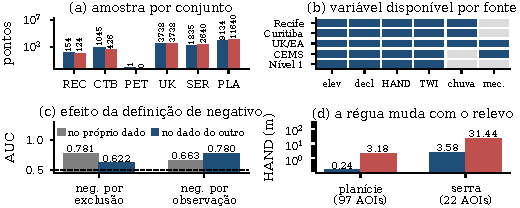
\includegraphics[width=0.97\columnwidth]{fig/fig2_datasets.pdf}
\caption{Três desafios, nos dados reais do projeto. (a) pontos por conjunto (SER
e PLA: serra e planície do EMS). (b) nenhuma fonte cobre todas as variáveis (azul = disponível).
(c) o modelo de maior AUC próprio é o que menos transfere. (d) HAND por classe de
relevo. Resolução nativa: 10\,m em Recife, 30\,m nas fontes externas, 3--10\,m no
Nível 1.}
\label{fig:datasets}
\end{figure}

% ------------------------------ TABELA I ------------------------------
\begin{table*}[!t]
\caption{Resumo de materiais e métodos; a Seção~II contextualiza cada linha.}
\label{tab:mm}
\centering
\renewcommand{\arraystretch}{0.95}
\scriptsize
\begin{tabular}{@{}>{\raggedright\arraybackslash}p{2.05cm}>{\raggedright\arraybackslash}p{7.6cm}>{\raggedright\arraybackslash}p{6.5cm}@{}}
\toprule
\textbf{Materiais} & \textbf{Descrição} & \textbf{Observações} \\
\midrule
Rótulo e evidência &
Positivos: SEDEC/Recife (154), SIAC 156/Curitiba (1.045), Diário Oficial,
ANA/SNIRH, Global Flood Database~\cite{tellman2021}. Negativo \emph{observado}:
Copernicus EMS, 25.249 pontos em 119 AOIs, mais a ativação EMSR720 no Rio Grande do
Sul (216,55\,km$^2$; 5,94:1). Negativo por \emph{exclusão qualificada}: Environment
Agency/UK, 7.476 pontos (3.738/3.738) em 201 eventos independentes &
Três níveis declarados por linha. Nenhuma região brasileira tem o nível de
observação; Curitiba passou a ter 114 pontos em exclusão qualificada
(critério do piloto inglês); o portão segue aberto para Recife e
Petrópolis. \\
Integração, variáveis e modelos &
Redução de toda fonte a tabela de pontos com procedência, resolução nativa, unidade
de agrupamento, classe de relevo e mecanismo. MDT PE3D 10\,m, Copernicus DEM GLO-30 e
SGB/CPRM; precipitação de fonte única Open-Meteo/ERA5-Land~\cite{munoz2021} em toda a
base, depois que a auditoria de confundimento por procedência retirou a mistura com
CHIRPS~\cite{funk2015}; Sentinel-1/2 e cobertura
do solo (auxiliares). Elevação, declividade, HAND~\cite{renno2008} e TWI~\cite{beven1979}
por D-infinity~\cite{tarboton1997}; pico e decaimento de chuva. Firth~\cite{firth1993}
como rota primária, não lineares como diagnóstico; \emph{gate} EPV~\cite{peduzzi1996},
\emph{bootstrap} de grupos $N$\,=\,1000, validação agrupada e \emph{walk-forward} &
Nenhuma variável derivada do rótulo, de escore ou de limiar; as orbitais \textbf{não
são causais}. Chuva recuperada para 99,99\% da base, de produto único, mas medida em
células de $\sim$11\,km enquanto o modelo compara pontos dentro do mesmo evento: nas
seis fontes ela não discrimina nessa escala, e entra como forçamento declarado, não
como propriedade do lugar. Quantas variáveis entram em cada ajuste é decisão de E3. A rota primária segue linear mesmo quando o
não linear tem AUC maior. \\
Serviço, ambiente e recursos &
API FastAPI com contrato de inferência e geoprocessamento sob demanda; \emph{model
card}~\cite{mitchell2019}; camada de explicação. Python 3.10 com \texttt{firthlogist},
\texttt{scikit-learn}, \texttt{interpret}, \texttt{rasterio}/GDAL, \texttt{whitebox} e
\texttt{pytest}; estação de 10 núcleos e 15,5\,GB, sem GPU; QGIS 3, GEE, Git &
A explicação lê o \emph{payload} já decidido. Recursos medidos: Firth 0,056\,s,
EBM 25,3\,s. \\
\bottomrule
\end{tabular}
\end{table*}

% =====================================================================
\section{Etapas do Projeto e Marcos Físicos}
\label{sec:etapas}

Cada etapa é encerrada por um arquivo conferível, produzido antes de a seguinte
começar; as datas da disciplina (Seção~\ref{sec:crono}) sincronizam, mas não
substituem esse critério.

\textbf{E0 e E1 --- Base consolidada e escopo congelado (concluídas).} Corpus,
governança de \emph{claims}, teste de ablação e definição de qual documento rege
o trabalho. \emph{Evidência}: artefatos versionados e uma afirmação de estado por
arquivo.

\textbf{E2 --- Integração e curadoria da evidência (M1, concluída).} Seis fontes
reduzidas a uma tabela única, com procedência, resolução, unidade de
agrupamento, classe de relevo e mecanismo por linha; recuperável geocodificado,
descarte do restante nomeado. \emph{Entregável}: base de conhecimento
geoespacial única, 65.070 pontos elegíveis ao ajuste fluvial, com as quatro
fontes do ajuste na mesma cadeia de derivação de terreno e Recife com fonte de
chuva única. \emph{Evidência}: contagem do que entra e do que sai por fonte
publicada; 21 de 22 testes de invariante passam nesta execução. No ambiente
fixado do projeto (Python 3.10, Tabela~\ref{tab:mm}) a reprodução bate exata;
a sensibilidade que resta é entre ambientes diferentes desse, ainda dependente
da versão de biblioteca.

\textbf{E3 --- Estimação e validação agrupada (M2, concluída).} Ajuste por classe
de relevo sobre a tabela única, com validação agrupada e aplicação cruzada.
\emph{Entregável}: coeficientes e desempenho por classe --- serra AUC 0,7916 com
\texttt{hand\_m} $-$1,44 [$-$3,11; $-$0,83]; planície 0,7245 com \texttt{hand\_m}
$-$2,10 [$-$2,78; $-$1,56] e \texttt{twi\_dinf} $+$0,40 [$+$0,33; $+$0,45]. O
modelo de planície aplicado à serra atinge 0,7957, acima do que a serra alcança
sozinha: a relação é a mesma nos dois terrenos, e o que separa é quão bem cada um
está estimado. \emph{Evidência}: EPV verificado antes de cada ajuste --- o
estrato íngreme tem 19 eventos positivos e comporta uma variável, não quatro ---,
sinais físicos conferidos depois, nenhum ajuste após olhar o teste.

\textbf{E4 --- \emph{Holdout} temporal (M3, concluída).} Janela expansiva sobre o
piloto inglês, 201 eventos em 110 datas entre 2000 e 2025, sem aquisição nova. O
corte temporal se aplica ao evento, que tem data; o negativo, amostrado por bloco
espacial, entra por sorteio declarado. \emph{Entregável}: oito cortes, todos na
faixa 0,70--0,88 fixada antes, AUC médio 0,7992, IC95 por \emph{bootstrap} de
grupos em cada um. \emph{Evidência}: cortes e trava de EPV declarados antes de
rodar; a mesma trava, aplicada às duas classes, mostra que Curitiba não sustenta
o teste --- 114 negativos contra 1.238 positivos ---, e isso fica como achado.
Vale para um país e para negativo por exclusão qualificada: refuta que o colapso
temporal seja do método, não prova estabilidade em serra tropical.

\textbf{E5 --- Aplicação às regiões brasileiras (M4, concluída).} A cadeia de
terreno já cobria as três regiões, então a grade saiu sem aquisição nova: 56.666
células em Recife, 65.275 em Curitiba e 172.015 em Petrópolis, a 120\,m.
\emph{Entregável}: mapa por região com maturidade declarada --- Recife
\texttt{mvp\_local}, Curitiba transferência caracterizada, Petrópolis
transferência sem referência local. A chuva entra como cenário, não como camada,
porque não varia nessa escala: ela desloca o escore e não muda o ordenamento.
\emph{Evidência}: distância de domínio medida variável a variável --- em
Curitiba a elevação está a 5,05 desvios do ajuste e nenhuma célula cai na faixa
vista, enquanto 91,3\% de Petrópolis cabe na faixa de HAND do modelo de serra.
Célula fora do domínio fica vazia no mapa em vez de receber escore baixo:
recusar não é o mesmo que dizer que ali é seguro.

\textbf{E6 --- Serviço e camada de explicação (M5, contrato executável).} O
contrato roda como função pura e auditável, com cinco portões avaliados em ordem
declarada; falta o transporte HTTP. \emph{Entregável}: cenários com resposta e
explicação correspondente --- Recife responde \texttt{ok} com maturidade
\texttt{mvp\_local} e o critério não atingido escrito na própria resposta;
Curitiba, transferência caracterizada com a extrapolação de elevação declarada;
Petrópolis, transferência sem referência local --- escore por semelhança de
terreno, nunca afirmação de acerto.
\emph{Evidência}: nenhuma explicação contradiz o \emph{payload} --- ela é montada
da mesma contribuição que entrou no escore, o que torna divergir impossível por
construção, e não por verificação posterior.

\textbf{E7 --- Congelamento, redação e pôster (M6--M7).} Testes completos,
repositório limpo e \emph{tag} de congelamento; depois disso, apenas redação
sobre artefatos congelados. \emph{Evidência}: cada número do manuscrito
rastreável a um arquivo.

\textbf{Riscos e rotas alternativas.} Declaradas agora, não improvisadas depois.
Em E2, fonte não harmonizável no prazo é documentada como descarte e não entra ---
o conjunto encolhe, o critério não. Em E4 a regra era publicar o desempenho
temporal como viesse, mesmo sem superar o acaso; ela foi cumprida onde doeu ---
o fold mais fraco e o estrato de Curitiba, que não sustenta o teste, estão
relatados. Em E6, se a explicação divergir do
\emph{payload}, a camada vira gerador por regras. Nenhuma altera a pergunta de
pesquisa.

% =====================================================================
\section{Cronograma}
\label{sec:crono}

O cronograma (Tabela~\ref{tab:crono}) cobre da submissão deste plano à
apresentação final e incorpora os \emph{checkpoints} da disciplina. As
durações partem do que o trabalho já feito levou de fato --- a integração da
Seção~\ref{sec:etapas} ocupou as duas primeiras quinzenas porque foi o tempo
real gasto para reduzir seis fontes a uma tabela única ---, e cada intervalo
carrega o resultado que a etapa correspondente busca (Seção~\ref{sec:etapas}
declara o \emph{entregável} e a \emph{evidência} de cada uma), não só a data
da disciplina. O estado da
arte já está em curso e permanece ativo até a redação. Sendo o trabalho
individual, as etapas se sobrepõem no tempo em vez de correr em paralelo entre
pessoas; foram identificadas de antemão sem que a ordem de conclusão seja
obrigatória --- o que muda de posição é a etapa, nunca o critério de evidência
que a encerra --- e a distribuição prevê folga porque pesquisa costuma exceder o
prazo. Os intervalos de 08/09 e 13/10 seguem sem tarefa nova; 24/11 e 01/12 são
contingência.

\begin{table}[!h]
\caption{Cronograma (quinzenas). E01 29/08, E02 31/10, E03 09/11, defesa 17/11.}
\label{tab:crono}
\centering
\renewcommand{\arraystretch}{0.88}
\setlength{\tabcolsep}{2.4pt}
\tiny
\begin{tabular}{@{}>{\raggedright\arraybackslash}p{1.85cm}ccccccc@{}}
\toprule
\textbf{Atividade} & \textbf{09--29} & \textbf{01--15} & \textbf{16--29} &
\textbf{30/09--} & \textbf{14--31} & \textbf{01--09} & \textbf{10--17} \\
 & \textbf{ago} & \textbf{set} & \textbf{set} & \textbf{13/10} &
\textbf{out} & \textbf{nov} & \textbf{nov} \\
\midrule
Estado da arte             & X & X & X &   &   &   &   \\
Integração (E2)            & X & X &   &   &   &   &   \\
Experimentação (E3--E4)    &   & X & X &   &   &   &   \\
Aplicação e serviço (E5--E6) &   &   & X & X &   &   &   \\
Análise                    &   &   & X & X & X &   &   \\
Auditoria (E7)             &   &   &   & X &   &   &   \\
Redação (E7)               &   &   &   & X & X & X &   \\
Pôster e defesa            &   &   &   &   &   & X & X \\
\midrule
\textit{Checkpoints} & \textbf{E01} & & & & \textbf{E02} & \textbf{E03} & \textbf{Def.} \\
\bottomrule
\end{tabular}
\end{table}

% =====================================================================
\fontsize{5.7}{6.2}\selectfont
\begin{thebibliography}{99}
\setlength{\itemsep}{0.4pt}
\setlength{\parskip}{0pt}

\bibitem{tellman2021}
B. Tellman \emph{et al.}, ``Satellite imaging reveals increased proportion of
population exposed to floods,'' \emph{Nature}, vol. 596, pp. 80--86, 2021.

\bibitem{ibge2018risco}
Instituto Brasileiro de Geografia e Estatística (IBGE), ``População em áreas
de risco no Brasil,'' IBGE, Rio de Janeiro, Brazil, Tech. Rep., 2018. [Online].
Available: \url{https://www.ibge.gov.br/geociencias/informacoes-ambientais/estudos-ambientais/21538-populacao-em-areas-de-risco-no-brasil.html}

\bibitem{renno2008}
C. D. Rennó \emph{et al.}, ``HAND, a new terrain descriptor using SRTM-DEM:
Mapping terra-firme rainforest environments in Amazonia,''
\emph{Remote Sensing of Environment}, vol. 112, no. 9, pp. 3469--3481, 2008.

\bibitem{beven1979}
K. J. Beven and M. J. Kirkby, ``A physically based, variable contributing area
model of basin hydrology,'' \emph{Hydrological Sciences Bulletin}, vol. 24,
no. 1, pp. 43--69, 1979.

\bibitem{tarboton1997}
D. G. Tarboton, ``A new method for the determination of flow directions and
upslope areas in grid digital elevation models,'' \emph{Water Resources
Research}, vol. 33, no. 2, pp. 309--319, 1997.

\bibitem{li2022pul}
W. Li \emph{et al.}, ``A positive-unlabeled learning algorithm for urban flood
susceptibility modeling,'' \emph{Land},
vol. 11, no. 11, art. 1971, 2022.

\bibitem{agostini2024}
G. Agostini, E. Pierson, and N. Garg, ``A Bayesian spatial model to correct
under-reporting in urban crowdsourcing,'' in \emph{Proc. AAAI}, vol. 38, 2024,
pp. 21\,888--21\,896.

\bibitem{firth1993}
D. Firth, ``Bias reduction of maximum likelihood estimates,''
\emph{Biometrika}, vol. 80, no. 1, pp. 27--38, 1993.

\bibitem{peduzzi1996}
P. Peduzzi \emph{et al.}, ``A simulation study of the number of events per
variable in logistic regression analysis,'' \emph{J. Clin. Epidemiol.}, vol. 49,
no. 12, pp. 1373--1379, 1996.

\bibitem{funk2015}
C. Funk \emph{et al.}, ``The climate hazards infrared precipitation with
stations,'' \emph{Scientific Data}, vol. 2, art. 150066, 2015.

\bibitem{munoz2021}
J. Muñoz-Sabater \emph{et al.}, ``ERA5-Land: a global reanalysis dataset for land
applications,'' \emph{Earth Syst. Sci. Data}, vol. 13, pp. 4349--4383, 2021.

\bibitem{mitchell2019}
M. Mitchell \emph{et al.}, ``Model cards for model reporting,'' \emph{Proc. ACM
FAT*}, pp. 220--229, 2019.

\end{thebibliography}

\end{document}
